\chapter{Methodology}
\label{chapter:Methodology}

For this thesis work, after an extensive literature review on crucial fields, concepts and technologies, we are ready to achieve the primary goal of this work.

This section presents the methodology applied to this project, from the work done to the work plan.

\section{Work Done}

This semester's work was mainly focused on state-of-the-art understanding and writing, going through a process of research and reading articles. The state-of-the-art objectives established in \autoref{chapter:Introduction} have been completed. These objectives are to study methodologies to build a conversational user interface, procedures to retrieve the databases of most interest and explore the definition of a study protocol. It was essential not only to learn more about the actual state of some technologies and concepts but also to get more into the project goal and requirements.

In terms of development, first, I built a prototype of an architecture, which is shown in figure \ref{fig_arch}, and then started the development.

\begin{figure}[ht]
    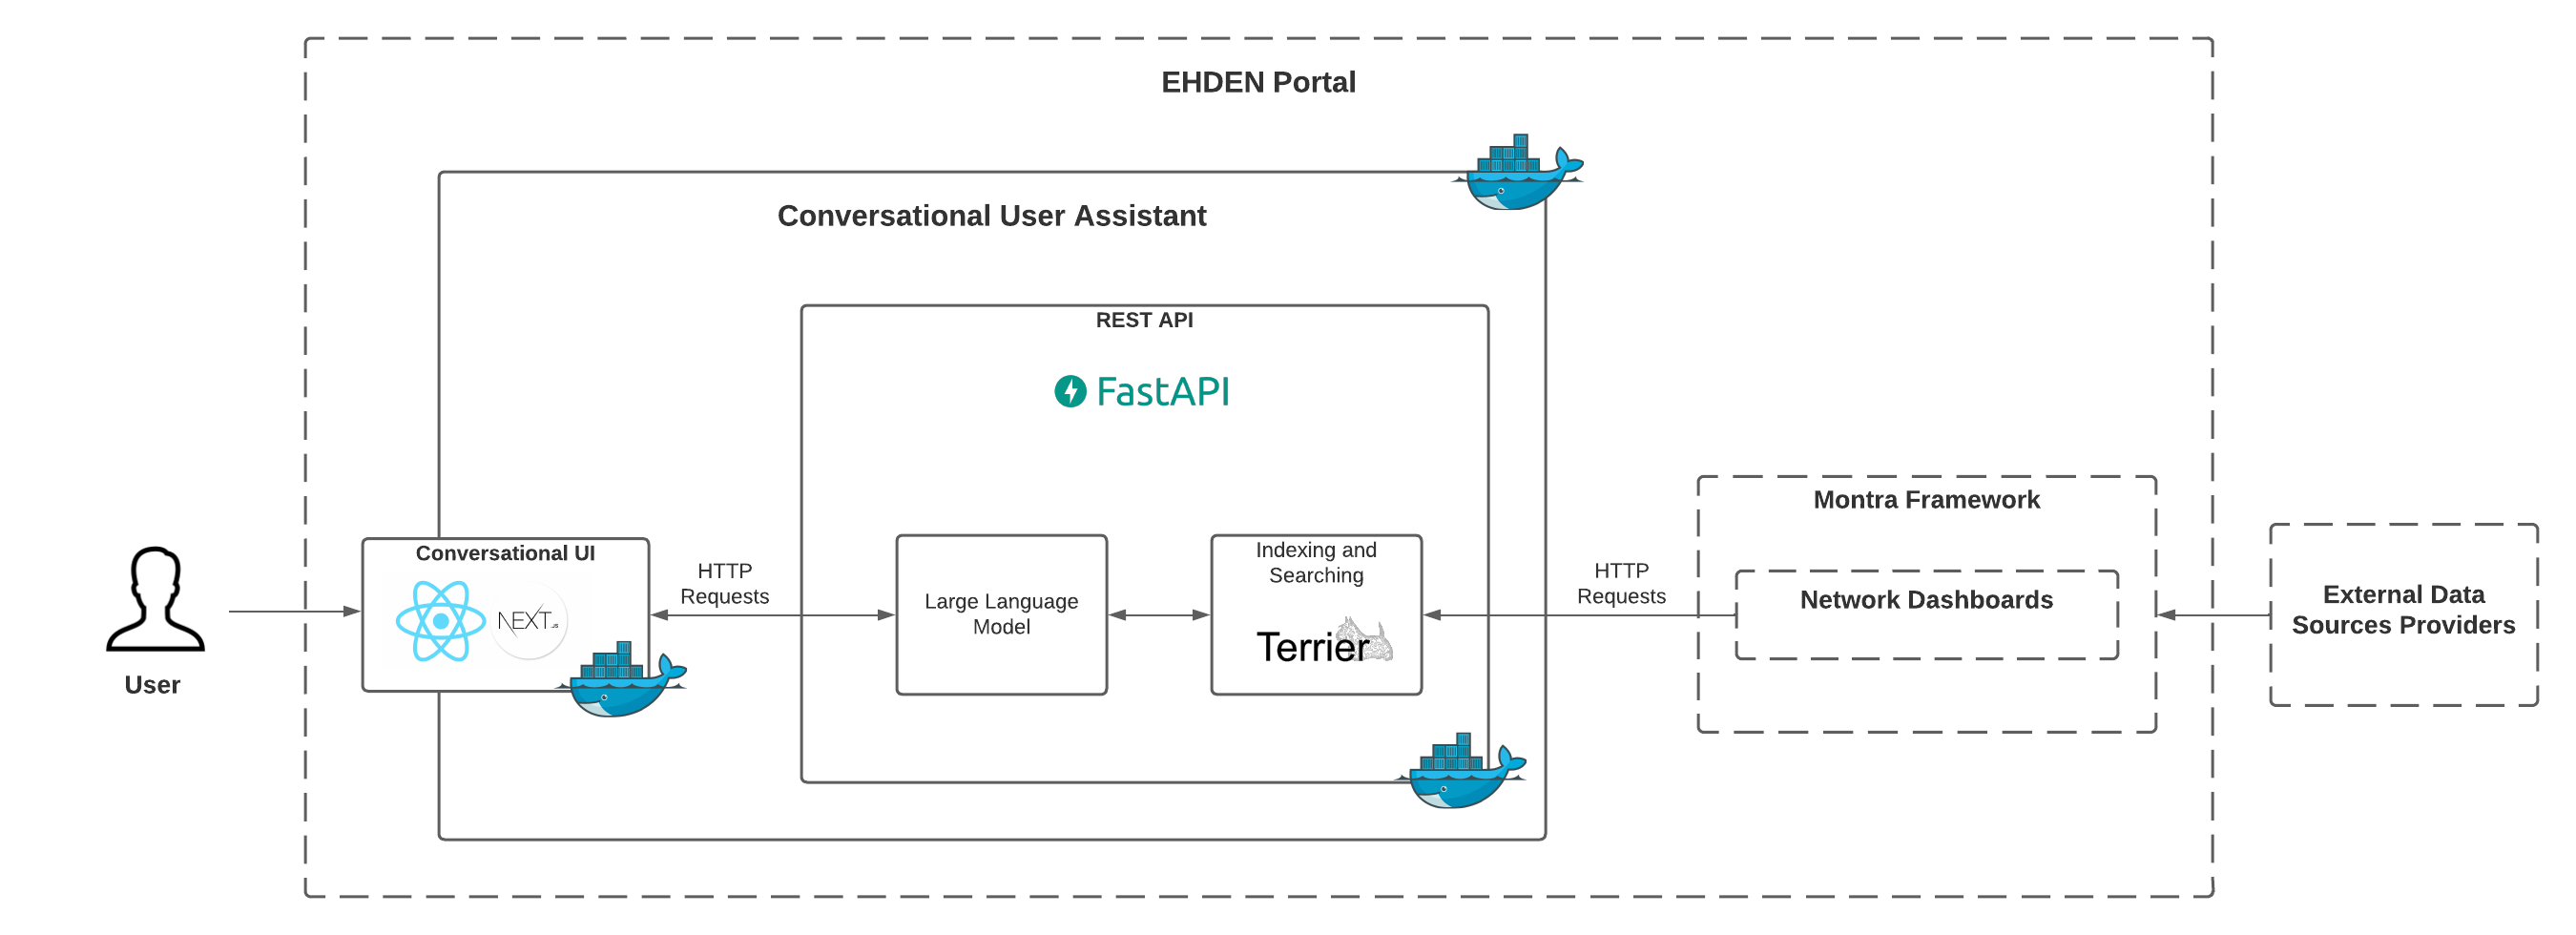
\includegraphics[width=16cm]{figs/methodology/arquitetura.png}
    \centering
    \caption{Architecture Proposal. Only the components with a solid line relate to the proposed work.}
    \label{fig_arch}
\end{figure}

I have developed a prototype of a chat-like interface using NextJS, a well-known ReactJS framework. Also, I have developed a REST API in FastAPI, a modern web framework based on Python. The interface and the API communicate between them through HTTP requests. The components of this application are deployed in Docker containers.

Beyond this, inside the backend module, I have started implementing and testing a {\bm} method to retrieve the best databases for a given user query. First, {\nlp} methods are applied to understand the plain-text query. For now, the {\nlp} method is in a very simple stage, because only tokenization, normalization, stemming and lemmatization are applied. Then, the {\bm} score is calculated between the query and the concepts of which database, making a database ranking. To implement the {\ir} technique, I am using the pyterrier library, and it could be changed to another library later if I discover another one more effective. The PyTerrier library facilitates the creation of a collection, allowing for the indexing and searching of data using a {\bm} method.
 
So, for now, the application developed can receive a user query through the frontend module and then, the backend module retrieves a rank of databases based on the query understanding. The chatbot interaction with the user is limited, as shown in figure \ref{fig_interface}. When the chatbot identifies a concept, he retrieves a list of clickable buttons of the ranked databases, indicating the database ID and its {\bm25} score. However, if it doesn't, it sends a pre-defined message.

\begin{figure}[ht]
    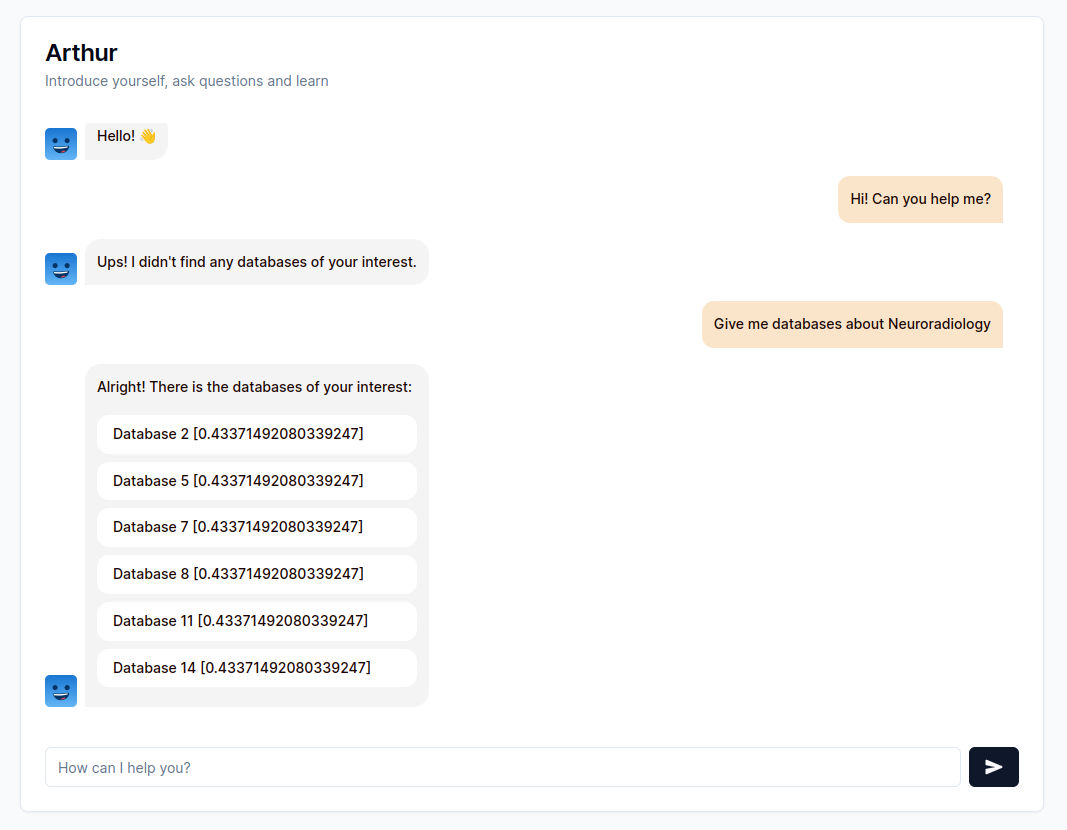
\includegraphics[width=12cm]{figs/methodology/interface.png}
    \centering
    \caption{Example of an interaction with the chatbot, showing the current state of the project.}
    \label{fig_interface}
\end{figure}



\section{Future work}

For the following months, I will continue the development of the database recommendation, based on {\bm}, improving some aspects, like concept linking. Also, test and improve this {\ir} implementation based on the testing results. 

After this, I will choose, implement, and fine-tune a {\llm} in order to guide the conversation to build the final query with the cohort definition structure. By doing this, the conversation flows naturally. Finally, test and improve the model based on the testing results.

The next step is integrating this system in the {\ehden} Portal and testing and validating the system. 

The documentation of the implementation and the respective steps taken will be carried out throughout its development.

The subsection \ref{workplan} presents a plan for all these tasks.


\section{Work Plan}
\label{workplan}

The following Gantt diagram, figure \ref{fig_gantt}, shows the work proposal for the following months. This diagram is divided into two semesters: the first refers to the work done in the first semester, and the second to the work proposed for the second semester.

\begin{figure}[ht]
    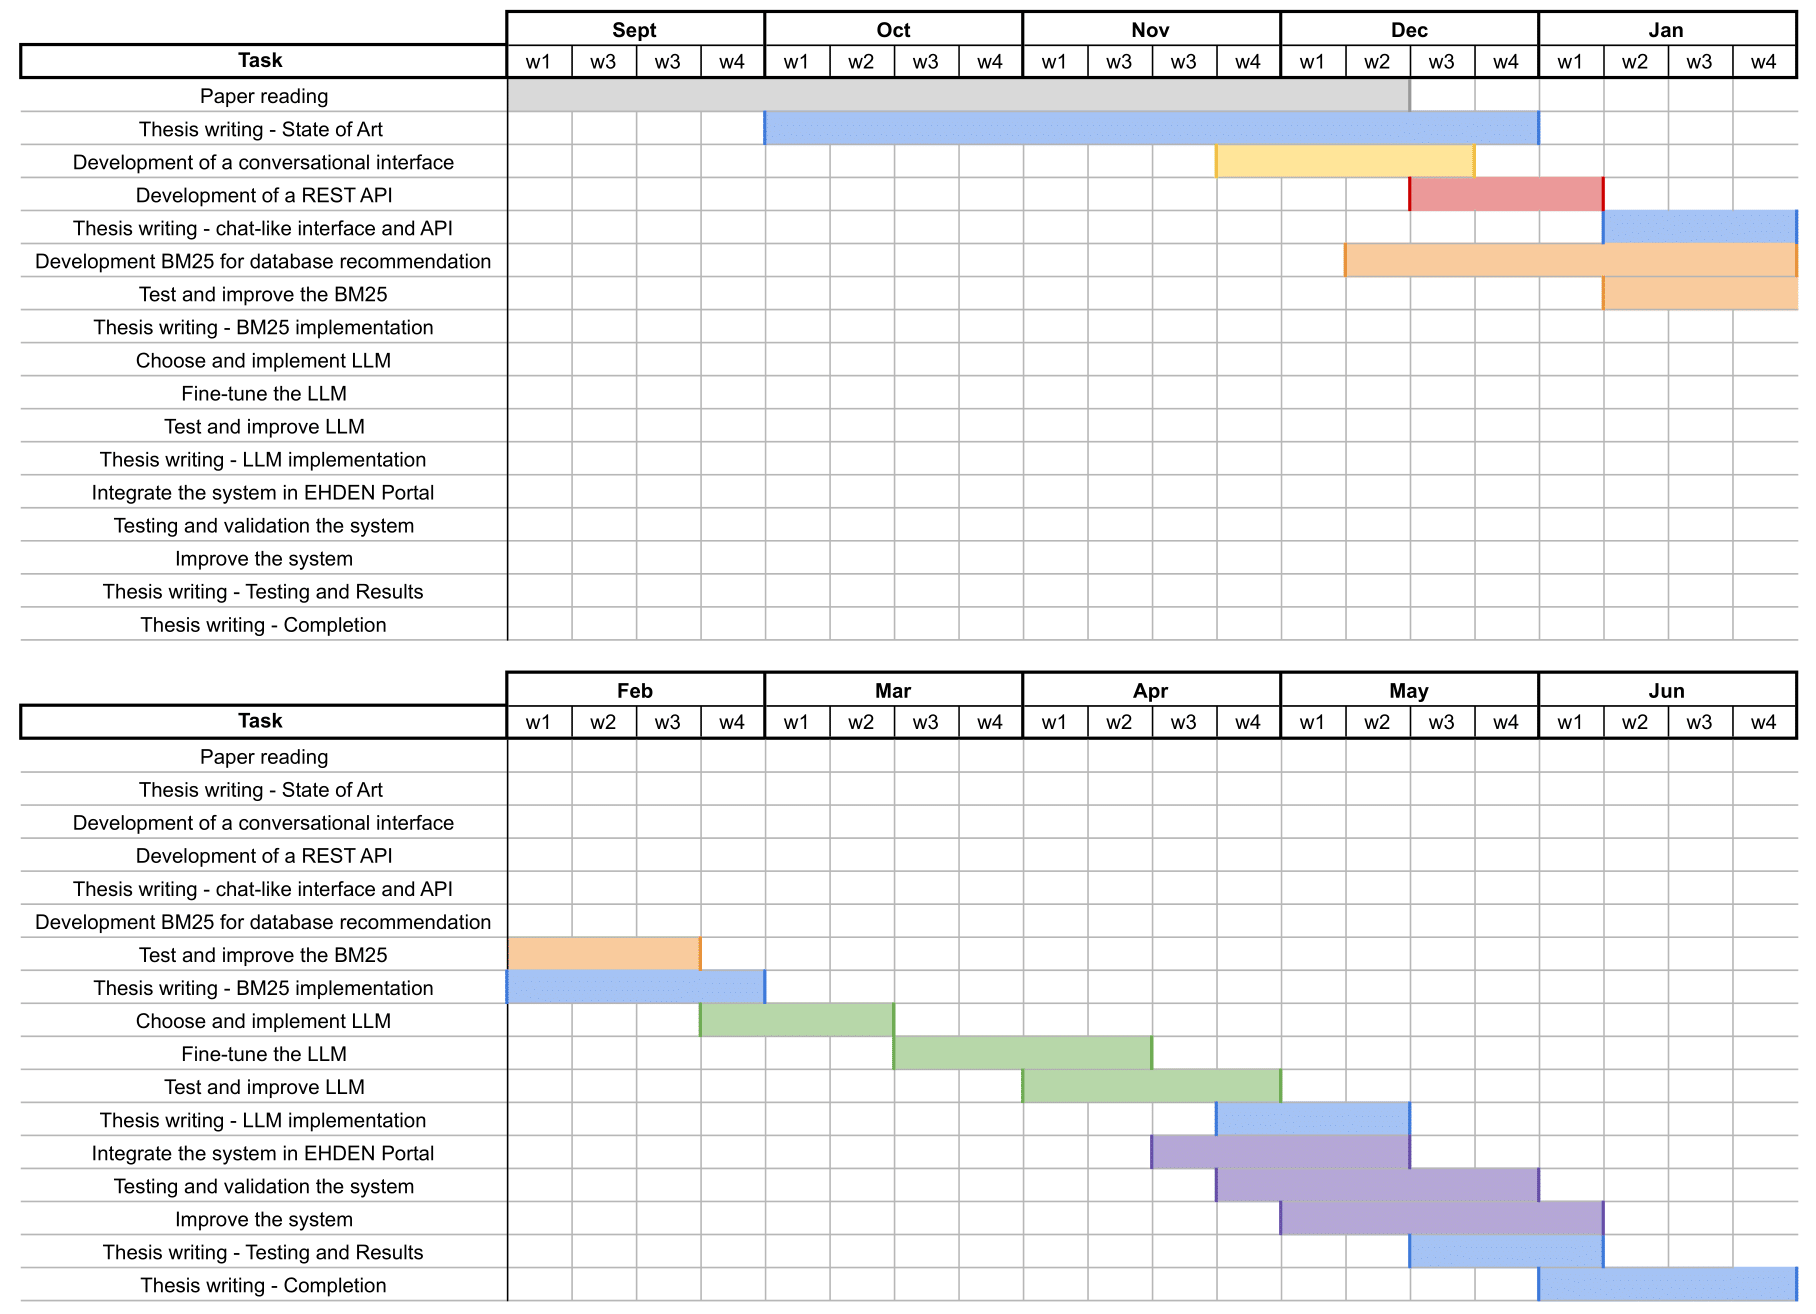
\includegraphics[width=16cm]{figs/methodology/diagram_gantt.png}
    \centering
    \caption{Proposal thesis work in a Gantt Diagram.}
    \label{fig_gantt}
\end{figure}